\chapter{Deployment}
Development of our application was done locally - using \textbf{Docker compose} to glue up three components necessary to sufficiently run our system - PHP runtime for web application, MySQL Database and Adminer. We have to, however, run our application in Kubernetes Cluster. \textbf{Service} and \textbf{Deployment} have to be written, Service for purposes of routing and taking care of container spawn addresses and Deployment to describe container replicas and approproate images. \textbf{Database} is run as separate entity within the Cluster.
\newline
\textbf{Running SwimmPair in Kubernetes Cluster:}
\par
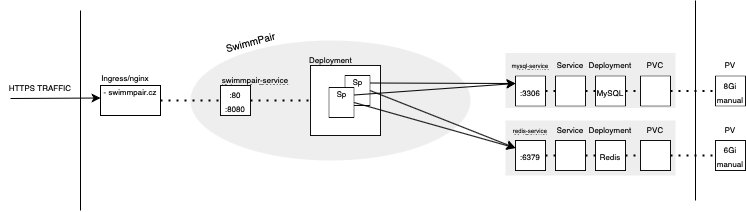
\includegraphics[scale=0.275]{img/swimmpair_deployment_k8s.png}
\section*{Dockerization of SwimmPair}
File called \textbf{Dockerfile} has to be created in the project folder.
\begin{lstlisting}
FROM thecodingmachine/php:7.4-v4-apache
COPY --chown=docker . /var/www/html
\end{lstlisting}
This image of Apache/PHP\footnote{Image \textbf{thecodingmachine/php:7.4-v4-apache}  by TheCodingMachine - \url{https://github.com/thecodingmachine/docker-images-php}} was chosen because it correctly dockerizes part of so-called LAMP stack. In order to build this image and push it into Dockerhub.com we run these commands:
\begin{lstlisting}
docker build -t stepanklos/swimmpair .
docker push stepanklos/swimmpair
\end{lstlisting}
This image is then pullable as stepanklos/swimmpair from Deployment.
\section*{Kubernetes}
We run 2 replicas on 2 Nodes in order to ensure reliability and uptime. 
\section*{Database and Redis}
As mentioned before, our application doesn't come with Database and Adminer, which have to be set up separately using persistent storage PV on which we write PVC and reference from deployment. 
